\section{\content{漢字的演變}{汉字的演变}}\label{section:evolution of chinese character}
\content{在本節,我們將了解漢字是如何從原始形態發展到如今之模樣的。我會從甲骨文開始,一路講到「二簡字」。}{在本节,我们将了解汉字是如何从原始形态发展到如今之模样的。我会从甲骨文开始,一路讲到“二简字”。}\par
\content{或許讀者會好奇,早已淘汰的甲骨文和廢棄的二簡字有什麼好學的?的確,本書作為「繁簡字體轉換手冊」並不是要教讀者怎麼寫甲骨文、金文、篆文以及二簡字。但是,現今通行的「繁體字」和「簡體字]作為字形演變的環節之一,須得放在整個漢字演變史中來看,才能令我們更深刻地理解文字是如何產生、如何發展的,其中又有什麼樣的規律。另外,二簡字在字形簡化方面同樣延續了這些規律,且比一簡字做得更加系統,並非沒有可取之處。因此,無論是繁體用戶學習簡體字,還是簡體用戶學習繁體字,本節內容都能讓我們有所收獲。}{或许读者会好奇,早已淘汰的甲骨文和废弃的二简字有什么好学的?的确,本书作为“繁简字体转换手册”并不是要教读者怎么写甲骨文、金文、篆文以及二简字。但是,现今通行的“繁体字”和“简体字”作为字形演变的环节之一,须得放在整个汉字演变史中来看,才能令我们更深刻地理解文字是如何产生、如何发展的,其中又有什么样的规律。另外,二简字在字形简化方面同样延续了这些规律,且比一简字做得更加系统,并非没有可取之处。因此,无论是繁体用户学习简体字,还是简体用户学习繁体字,本节内容都能让我们有所收获。}\par
\content{遺憾的是,筆者並非古漢語及書法方面的專家,所以我講解的內容也往往只能浮於表面,且難免出現錯誤和缺漏。不過我還是會盡力為讀者提供可靠的資訊及參考資料。}{遗憾的是,笔者并非古汉语方面的专家,所以我讲解的内容也往往只能浮于表面,且难免出现错误和缺漏。不过我还是会尽力为读者提供可靠的信息及参考资料。}\par
\subsection{\content{書寫工具的沿革}{书写工具的沿革}}
\begin{boxquote}{\content{《後漢書·宦者列傳》}{《后汉书·宦者列传》}}
	\content{自古書契多編以竹簡,其用縑帛者謂之為紙。縑貴而簡重,並不便於人。倫乃造意,用樹膚、麻頭及敝布、魚網以為紙。}{自古书契多编以竹简,其用缣帛者谓之为纸。缣贵而简重,并不便于人。伦乃造意,用树肤、麻头及敝布、鱼网以为纸。}
\end{boxquote}
\content{最早發現的\textbf{甲骨文}都是用刀之類的鋒利物品刻在「甲骨」之上的。「甲骨」是通稱,「甲」一般指龜甲,「骨」一般指牛骨。它們都不易腐爛,能在地下長期保存,只要能被有心人發現,便可以帶著一個古老時代的謎團重見天日。}{最早发现的\textbf{甲骨文}都是用刀之类的锋利物品刻在“甲骨”之上的。“甲骨”是通称,“甲”一般指龟甲,“骨”一般指牛骨。它们都不易腐烂,能在地下长期保存,只要能被有心人发现,便可以带着一个古老时代的谜团重见天日。}\par
\content{晚清金石學家王懿榮便是這樣的有心人。他偶然地從中藥材「龍骨」上發現了形如文字的符號,並斷定這就是早期的漢文字。在隨後的一百多年裡,歷代學者發掘和釋讀出了越來越多的甲骨文,這些甲骨文內容又與史書互相佐證,為人們還原出了更豐富的殷商歷史面貌。}{晚清金石学家王懿荣便是这样的有心人。他偶然地从中药材“龙骨”上发现了形如文字的符号,并断定这就是早期的汉文字。在随后的一百多年里,历代学者发掘出了越来越多的甲骨文,这些甲骨文内容又与史书互相佐证,为人们还原出了更丰富的殷商历史面貌。}\par
\begin{wrapfigure}{O}{.46\textwidth}
	\begin{subcaptionblock}{.15\textwidth}
		\centering
		
\includegraphics[width=\textwidth]{甲骨文/史}
		\caption{\content{史}{史}}
	\end{subcaptionblock}
	\begin{subcaptionblock}{.15\textwidth}
		\centering
		
\includegraphics[width=\textwidth]{甲骨文/冊}
		\caption{\content{冊}{册}}
	\end{subcaptionblock}
	\begin{subcaptionblock}{.15\textwidth}
		\centering
		
\includegraphics[width=\textwidth]{甲骨文/典}
		\caption{\content{典}{典}}
	\end{subcaptionblock}
	\caption{}
	\label{figure:甲骨文中的「史」「冊」「典」}
\end{wrapfigure}
\content{較近的考古證據則表明,商代人的主要書寫工具並不是甲骨,而是\textbf{毛筆和竹簡}\footnote{參見《了不起的文明現場:跟著一線考古隊長穿越歷史》李零等著。}。我們看\cref*{figure:甲骨文中的「史」「冊」「典」},甲骨文中「史」字描繪的是手拿筆桿寫字的模樣;「冊」字則像一排竹簡串起來的樣子;「典」字更形象,它描繪的是雙手端著竹簡的模樣。}{较近的考古证据则表明,商代人的主要书写工具不是甲骨,而是\textbf{毛笔和竹简}\footnote{参见《了不起的文明现场:跟著一线考古队长穿越历史》李零等著。}。我们看\cref*{figure:甲骨文中的「史」「冊」「典」},甲骨文中“史”字描绘的是手拿笔杆写字的模样;“册”字则像一排竹简串起来的样子;“典”字更形象,它描绘的是双手端着竹简的模样。}\par
\content{毛筆、竹簡要比龜甲、兽骨更易獲取,因此它的用途也就更「日常化」。但可惜的是,竹簡易腐,考古界至今也難以得到三千多年前的有字竹簡,所以罕有直接證據能夠說明當時竹簡的用途。}{毛笔、竹简要比龟甲、兽骨更易获取,因此它的用途也就更“日常化”。但可惜的是,竹简易腐,考古界至今也难以得到三千多年前的有字竹简,所以罕有直接证据能够说明当明当时竹简的用途。}\par
\content{而在同一時期,青銅器則要比甲骨更難獲取。因此青銅器上的\textbf{金文}就必須用來記錄最重要的事情,萬萬不能寫流水賬。就從出土文物來看,商代甲骨文多用於記錄祭祀、戰爭、狩猎、歷法、天象等,內容繁多;但商朝青銅器上的銘文就顯得惜字如金,大多只是記錄鑄者或其祖先的名稱,僅有廖廖幾字。}{而在同一时期,青铜器则要比甲骨更难获取。因此青铜器上的\textbf{金文}就必须用来记录最重要的事情,万万不能写流水账。就从出土文物来看,商代甲骨文多用于记录祭祀、战争、历法、天象等,内容繁多;但商朝青铜器上的铭文就显得惜字如金,大多只是记录铸者或其祖先的名称,仅有廖廖几字。}\par
\content{及至西周,乃至春秋、戰國,青銅器工藝漸臻成熟,產量也越來越高,人們對於金文的使用也不再那樣吝嗇。於是,舉凡王公貴族之事,無論大小,都可以記錄在青銅器上,金文的發展便在周代達到最盛;而殷商甲骨文則隨著商代的覆滅,一並失傳。}{及至西周,乃至春秋、战国,青铜器工艺渐臻成熟,产量也越来越高,人们对于金文的使用也不再那样吝啬。于是,举凡王公贵族之事,无论大小,都可以记录在青铜器上,金文的发展便在周代达到最盛;而殷商甲骨文则随着商代的覆灭,一并失传。}\par
\begin{wrapfigure}{O}{.4\textwidth}
	\centering
	\vspace{-1em}
	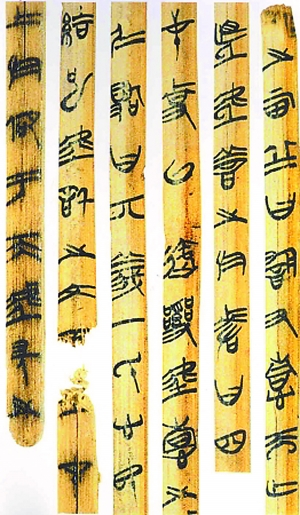
\includegraphics[width=.3\textwidth]{孔子詩論竹簡.jpg}
	\caption{\content{《孔子詩論》竹簡片段}{《孔子诗论》竹简片段}}
	\label{figure:《孔子詩論》竹簡片段}
\end{wrapfigure}
\content{春秋、戰國人也用竹簡寫字。\cref*{figure:《孔子詩論》竹簡片段}便是《孔子詩論》的竹簡書,其間所寫的文字應當是大篆的一種。除了竹簡之外,人們也偶爾使用\textbf{絲綢}(古稱「帛」)來書寫——這大概是中國歷史上最早的「紙」了。但絲綢既不像竹簡那樣廉價,又不像青銅器那樣容易保存,所以始終沒有普及開來。東漢蔡倫改進造紙術後,紙張的生產成本大大降低,這才逐漸取代笨重的竹簡,成為兩千多年來的主流書寫工具。}{春秋、战国人也用竹简写字。\cref*{figure:《孔子詩論》竹簡片段}便是《孔子诗论》的竹简书,其间所写的文字应当是大篆的一种。除了竹简之外,人们也偶尔使用\textbf{丝绸}(古称“帛”)来书写——这大概是中国历史上最早的“纸”了。但丝绸既不像竹简那样廉价,又不像青铜器那样容易保存,所以始终没有普及开来。东汉蔡伦改进造纸术后,纸张的生产成本大大降低,这才逐渐取代笨重的竹简,成为两千多年来的主流书写工具。}\par
\content{戰國時期雖有毛筆,但尚不成熟,很少被人使用。當時的人們在竹簡上寫字,通常是用竹簽點漆,或是用刀篆刻——這兩類書寫工具都算是「硬筆」。戰國末期的秦將蒙恬改進了毛筆,才使毛筆逐漸取代硬筆的地位,成為主流的書寫工具。}{战国时期虽有毛笔,但尚不成熟,很少被人使用。当时的人们在竹简上写字,通常是用竹签点漆,或是用刀篆刻——这两类书写工具都算是“硬笔”。战国末期的秦将蒙恬改进了毛笔,才使毛笔逐渐取代硬笔的地位,成为主流的书写工具。}\par
\content{毛筆和紙張對漢字演變有著重大意義。毛筆運筆靈活,細節豐富,變化無窮,書寫的多樣性比硬筆高出一個檔次,於是後世各種風格的楷書、行書、草書層出不窮。廉價的紙張對於文人墨客來說,同樣不可或缺。相傳王羲之每日練完書法都在住處附近的池中洗筆,經年累月竟把池水洗黑。若他是用絲綢練字的話,恐怕還沒練成就已傾家蕩產了。}{毛笔和纸张对汉字演变有着重大意义。毛笔运笔灵活,细节丰富,变化无穷,书写的多样性比硬笔高出一个档次,于是后世各种风格的楷书、行书、草书层出不穷。廉价的纸张对于文人墨客来说,同样不可或缺。相传王羲之每日练完书法都在住处附近的池中洗笔,经年累月竟把池水洗黑。若他是用丝绸写字的话,恐怕还没练成就已倾家荡产了。}\par
\content{到了現代,隨著硬筆生產技術的提高和人們對書寫效率的要求,硬筆又占據了主流市場;而紙張的地位則從未被撼動。不過現代人還多了一套「書寫工具」,那就是——鍵盤、熒屏和印表機。}{到了现代,随着硬笔生产技术的提高和人们对书写效率的要求,硬笔又占据了主流市场;而纸张的地位则从未被撼动。不过现代人还多了一套“书写工具”,那就是——键盘、屏幕和打印机。}\par
\subsection{\content{印刷術的發展}{印刷术的发展}}
\begin{boxquote}{\content{《農書·麻苧門》}{《农书·麻苎门》}}
	\content{後世有人別生巧技,以鐵為印盔,界行內用稀瀝青澆滿,冷定取平。火上再行煨化,以燒熟瓦字,排于行內,作活字印板。}{后世有人别生巧技,以铁为印盔,界行内用稀沥青浇满,冷定取平。火上再行煨化,以烧熟瓦字,排于行内,作活字印板。}
\end{boxquote}
\content{印刷與手寫大不相同。我們談書法中的「字體」,最常講的是「楷書」「行書」「草書」這些概念;但談及電腦字體和印刷字體,最常講的卻是「明體(宋體)」「楷體」「黑體」「仿宋體」這些概念。本小節我們只聚焦於印刷;至於電腦漢字,我將單獨撰寫一節內容來介紹它。}{印刷与手写大不相同。我们谈书法中的“字体”,最常讲的是“楷书”“行书”“草书”这些概念;但谈及电脑字体和印刷字体,最常讲的却是“宋体(明体)”“楷体”“黑体”“仿宋体”这些概念。本小节我们只聚焦于印刷;至于电脑汉字,我将单独撰写一节内容来介绍它。}\par
\content{最早的印刷工具當屬\textbf{印章}。古人用刀具將文字反刻在銅塊、銀塊、玉塊等材料上,然後就可以用它蘸取印泥(通常是紅色的),印下油墨,這就是一種「印刷」了。}{最早的印刷工具当属\textbf{印章}。古人用刀具将文字反刻在铜块、银块、玉块等材料上,然后就可以用它蘸取印泥(通常是红色的),印下油墨,这就是一种“印刷”了。}\par
\begin{wrapfigure}{O}{.51\textwidth}
	\centering
	\begin{subcaptionblock}{.25\textwidth}
		\centering
		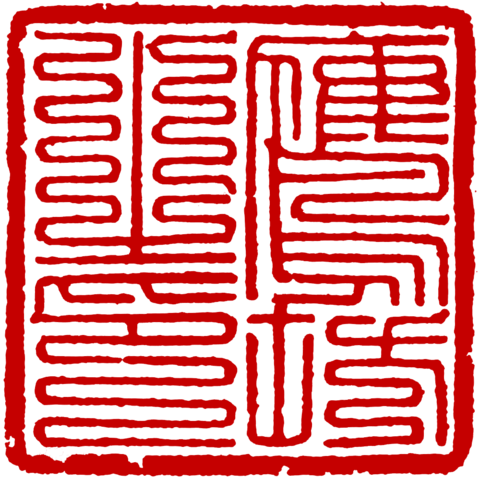
\includegraphics[width=\textwidth]{九疊篆印章「鷹坊之印」.png}
		\caption{\content{九疊篆陽文印}{九叠篆阳文印}}
		\label{figure:九疊篆陽文印「鷹坊之印」}
		\footnotesize{\color{darkgray}\content{「鷹坊之印」}{“鹰坊之印”}}
	\end{subcaptionblock}
	\begin{subcaptionblock}{.25\textwidth}
		\centering
		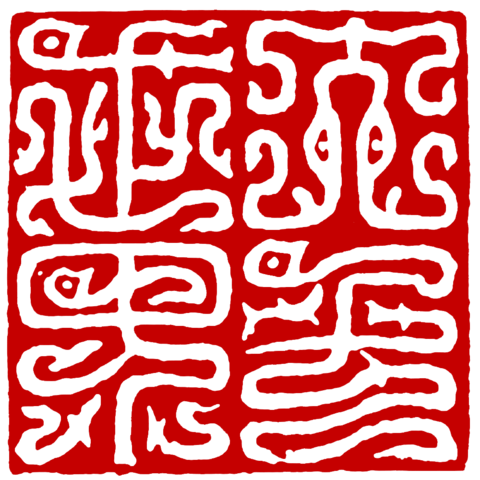
\includegraphics[width=\textwidth]{鳥蟲篆印章「大千世界」.png}
		\caption{\content{鳥蟲篆陰文印}{鸟虫篆阴文印}}
		\label{figure:鳥蟲篆陰文印「大千世界」}
		\footnotesize{\color{darkgray}\content{「大千世界」}{“大千世界”}}
	\end{subcaptionblock}
	\caption{}
	\vspace{-1em}
\end{wrapfigure}
\content{根據印文的凹凸,我們可以把印章分為「陽文印」和「陰文印」。陽文印是文字部分凸起,所以印出來得到的是白底紅字(\cref*{figure:九疊篆陽文印「鷹坊之印」});陰文印是文字部分凹下,所以印出來得到的是紅底白字(\cref*{figure:鳥蟲篆陰文印「大千世界」})。}{根据印文的凹凸,我们可以把印章分为“阳文印”和“阴文印”。阳文印是文字部分凸起,所以印出来得到的是白底红字(\cref*{figure:九疊篆陽文印「鷹坊之印」});阴文印是文字部分凹下,所以印出来得到的是红底白字(\cref*{figure:鳥蟲篆陰文印「大千世界」})。}\par
\content{印章從春秋戰國時期就開始流行了。當時的主要文字是大篆,所以印章普遍使用篆文刻成。後世也往往使用篆文,而很少有使用楷書、行書、草書來刻章的——可能是文人尚古的風氣使然,也可能是篆文顯得嚴肅、莊重。但筆者認為還有一個關鍵因素:用刀這樣的硬筆來刻寫毛筆字,實在是不容易。}{印章从春秋战国时期就开始流行了。当时的主要文字是大篆,所以印章普遍使用篆文刻成。后世也往往使用篆文,而很少有使用楷书、行书、草书来刻章的——可能是文人尚古的风气使然,也可能是篆文显得严肃、庄重。但笔者认为还有一个关键因素:用刀这样的硬笔来刻写毛笔字,实在是不容易。}\par
\content{\textbf{雕版印刷}則是真正意義上的「印刷術」。隋唐時期,人們先用毛筆把文字寫在特別薄的宣紙上,然後把紙張反貼在木板上,再由雕刻師傅挖掉沒有墨跡的地方,這樣就造好了一塊「印版」。印刷時,只需在印版上刷好墨,再鋪紙按壓,即可完成一次印刷。所以在這一時期,印刷品上所印的自然是楷書。}{\textbf{雕版印刷}则是真正意义上的“印刷术”。隋唐时期,人们先用毛笔把文字写在特别薄的宣纸上,然后把纸张反贴在木板上,再由雕刻师傅挖掉没有墨迹的地方,这样就造好了一块“印版”。印刷时,只需要印版上刷好墨,再铺纸按压,即可完成一次印刷。所以在这一时期,印刷品上所印的自然是楷书。}\par
\content{宋朝及以後,印刷業空前繁榮,書籍、紙鈔等印刷品開始普及到庶民階層。為了應對爆發式增長的印刷需求,印刷業也急需改進原本的工藝和流程。刻字工們不再照著宣紙上的墨跡刻版了,而是乾脆徒手刻字,以求速成。}{宋朝及以后,印刷业空前繁荣,书籍、纸钞等印刷品开始普及到庶民阶层。为了应对爆发式增长的印刷需求,印刷业也急需改进原本的工艺和流程。刻字工们不再照着纸上的墨迹刻版了,而是干脆徒手刻字,以求速成。}\par
\content{但徒手刻字還面臨一個很大的問題:要用\cref*{figure:徒手刻版}那樣的硬筆還原出毛筆的細節,實在是費時費力,事倍功半。所以從宋朝開始,刻字工們逐漸改變了楷書的筆畫,化曲為直,務求易於刻制。到明朝初年,印刷界已經產生了一種較為成熟的字體——\textbf{明體(也稱宋體)}。這是印刷字體與書法字體分道揚鑣的開始。}{但徒手刻字还面临一个很大的问题:要用\cref*{figure:徒手刻版}那样的硬笔还原出毛笔的细节,实在是费时费力,事倍功半。所以从宋朝开始,刻字工们逐渐改变了楷书的笔画,化曲为直,务求易于刻制。到明朝初年,印刷界已经产生了一种较为成熟的字体——\textbf{宋体(也称明体)}。这是印刷字体与书法字体分道扬镳的开始。}\par
\begin{figure}[H]
	\centering
	\begin{tikzpicture}
		\definecolor{seal red}{HTML}{C50000}
		\node[inner sep=0pt](main)at(-.78,0){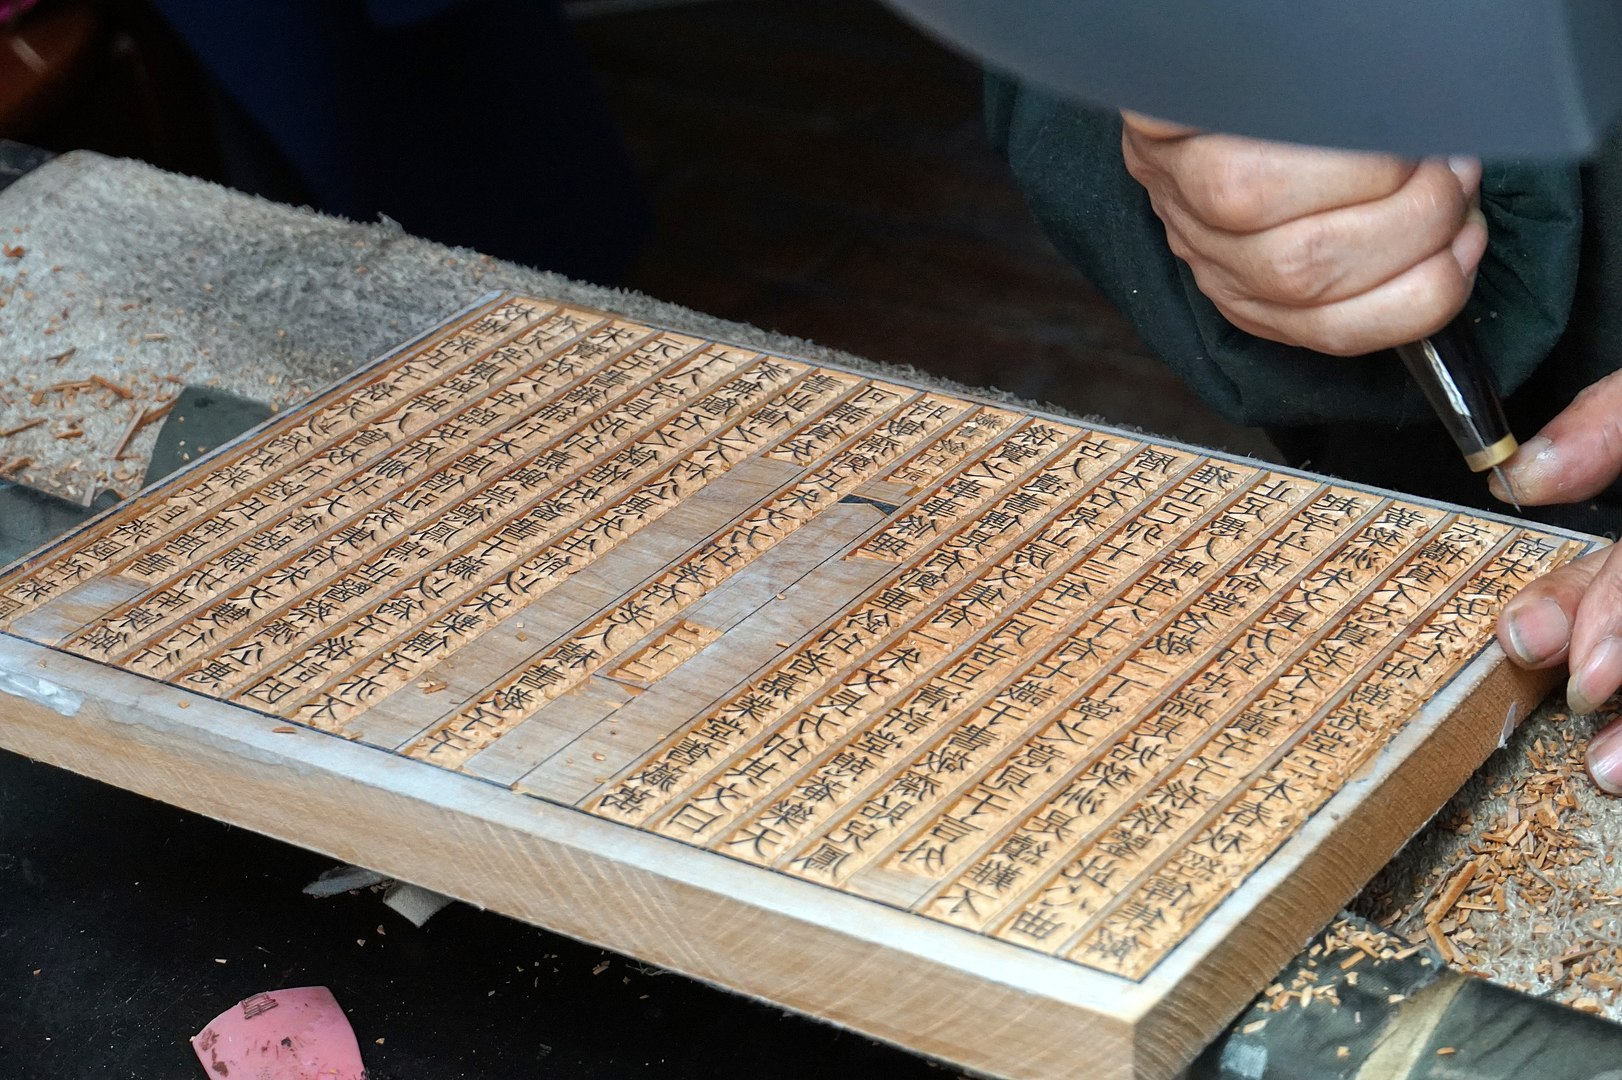
\includegraphics[width=.5\textwidth]{徒手刻版.jpg}};
		\begin{scope}
			\clip(8,0)circle(2.5);
			\node[inner sep=0pt]at(-8.4,-1.6){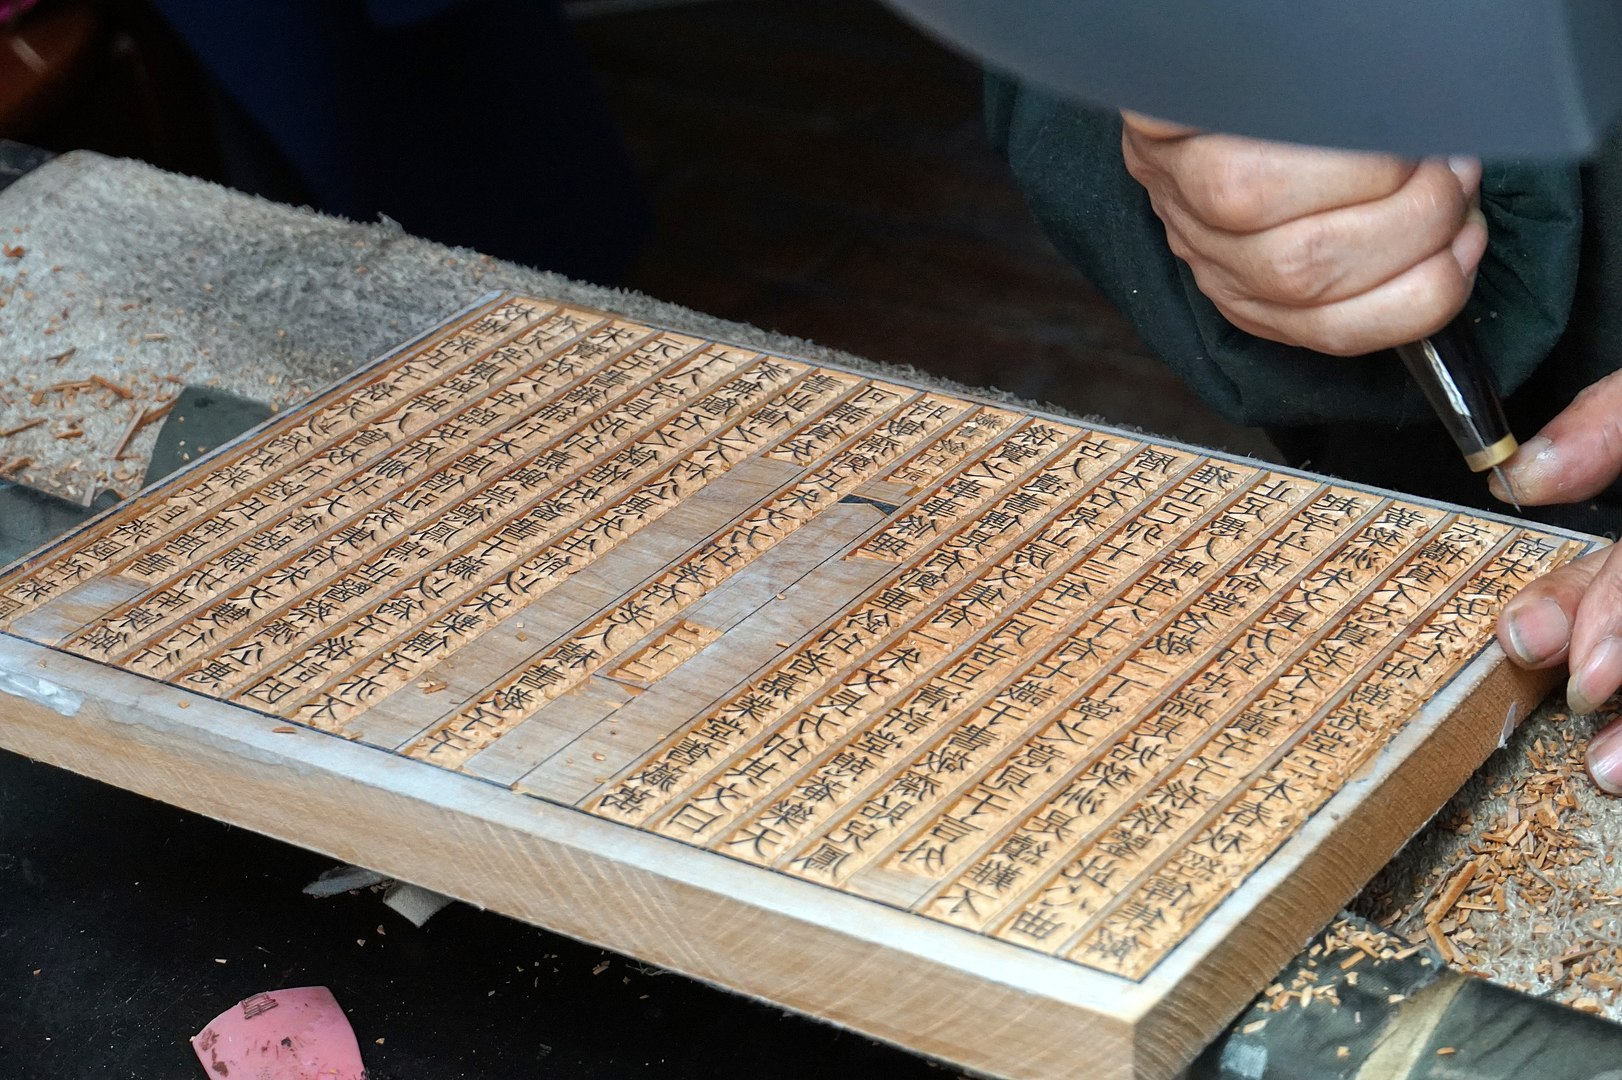
\includegraphics[width=2.5\textwidth]{徒手刻版.jpg}};
		\end{scope}
		\node[draw,circle,seal red,thin,minimum size=1cm](small)at(2.5,.32){};
		\node[draw,circle,seal red,minimum size=5cm](big)at(8,0){};
		\draw[dashed,seal red](tangent cs:node=small,point={(big.south)},solution=2)--(tangent cs:node=big,point={(small.south)},solution=1);
		\draw[dashed,seal red](tangent cs:node=small,point={(big.north)},solution=1)--(tangent cs:node=big,point={(small.north)},solution=2);
	\end{tikzpicture}
	\caption{\content{徒手刻版}{徒手刻版}}
	\label{figure:徒手刻版}
\end{figure}
\content{北宋的畢昇發明了\textbf{活字印刷術}。這種方法不再是以版面為單位來印刷,而是以漢字為單位來印刷。刻字工只需要預先刻好所需文字,把它們做成字模(稱為「活字」),就可以任意取用。於是,昨天用來印《水滸傳》的字,明天還能取下來印《紅樓夢》,而不需要另外刻版,這是何等方便的事!}{北宋的毕昇发明了\textbf{活字印刷术}。这种方法不再是以版面为单位来印刷,而是以汉字为单位来印刷。刻字工只需要预先刻好所需文字,把它们做成字模(称为“活字”),就可以任意取用。于是,昨天用来印《水浒传》的字,明天还能取下来印《红楼梦》,而不需要另外刻版,这是何等方便的事!}\par
\content{但活字印刷也有一些缺點,這使得它在古代的中國並不如雕版印刷那樣流行。比如說,活字印刷只能刻印文字,而雕版印刷既可以刻印文字,又可以刻印圖像。那麼,若是要印全本繡像《金瓶梅》的話,活字印刷就顯得有些捉襟見肘了。}{但活字印刷也有一些缺点,这使得它在古代的中国并不如雕版印刷那样流行。比如说,活字印刷只能刻印文字,而雕版印刷既可以刻印文字,又可以刻印图像。那么,若是要印全本绣像《金瓶梅》的话,活字印刷就显得有些捉襟见肘了。}\par
\content{更致命的問題是,漢字數量繁多,活字印刷前需要預先投入巨大的工作量,才能準備好充足的活字\footnote{而且很多常用字可能在同一版面出現幾次甚至十幾次,所以需要有多個備用字,這又是很大的工作量。}。但歐文只有幾十個字母,制作活字的工作量要小很多,因此活字印刷術才能在歐洲大放異彩,從而推動了歐洲印刷的工業化進程。}{更致命的问题是,汉字数量繁多,活字印刷前需要预先投入巨大的工作量,才能准备好充足的活字\footnote{而且很多常用字可能在同一版面出现几次甚至十几次,所以需要有多个备用字,这又是很大的工作量。}。但欧文只有几十个字母,制作活字的工作量要小很多,因此活字印刷术才能在欧洲大放异彩,从而推动了欧洲的工业化进程。}\par
\content{現代印刷術已經不以「字」為單位了——甚至說,根本不需要「字」這個概念。印表機的眼中只有數以億計的密密麻麻的點,而它要做的就是在正確的點位加上正確的墨。於是,無論文字、圖畫、數學式,還是什麼奇奇怪怪的符號,印表機都可以在幾秒之內搞定,就像魔術一樣。}{现代印刷术已经不以“字”为单位了——甚至说,本不需要“字”这个概念。打印机的眼中只有数以亿计的密密麻麻的点,而它要做的就是在正确的点位加上正确的墨。于是,无论文字、图画、数学式,还是什么奇奇怪怪的符号,打印机都可以在几秒之内搞定,就像魔术一样。}\par
\content{電腦和印表機的出現打破了硬筆的局限,使人類對字體細節的控制能力提高到了前所未有的水平。短短幾十年間,中文印刷界就出現了各種各樣不同的黑體、圓體、仿宋體,以及富有特色的綜藝體、疊圓體等——當然還有在台灣風靡一時的康熙字典體。}{电脑和打印机的出现打破了硬笔的局限,使人类对字体细节的控制能力提高到了前所未有的水平。短短几十年间,中文印刷界就出现了各种各样不同的黑体、圆体、仿宋体,以及富有特色的综艺体、叠圆体等——当然还有在台湾风靡一时的康熙字典体。}\par
\subsection{\content{字形的變化}{字形的变化}}
\begin{boxquote}{\content{《說文解字·序》}{《说文解字·序》}}
	\content{是時,秦燒滅經書,滌除舊典。大發吏卒,興戍役。官獄職務繁,初有隸書\footnotemark,以趣約易,而古文由此絕矣。}{是时,秦烧灭经书,涤除旧典。大发吏卒,兴戍役。官狱职务繁,初有隶书\footnotemark,以趣约易,而古文由此绝矣。}
\end{boxquote}
\footnotetext{\content{現代學者一般認為,隸書的原型在戰國時代就已存在。《說文》說秦朝「初有隸書」是不對的。}{现代学者一般认为,隶书的原型在战国时代就已存在。《说文》说秦朝“初有隶书”是不对的。}}
\subsubsection*{\content{何為「古文」?}{何为“古文”?}}
\begin{wrapfigure}{O}{8.6cm}
	\centering
	\begin{boxhorizontalcompare}[width=8.6cm,lefthand width=4.2cm]
		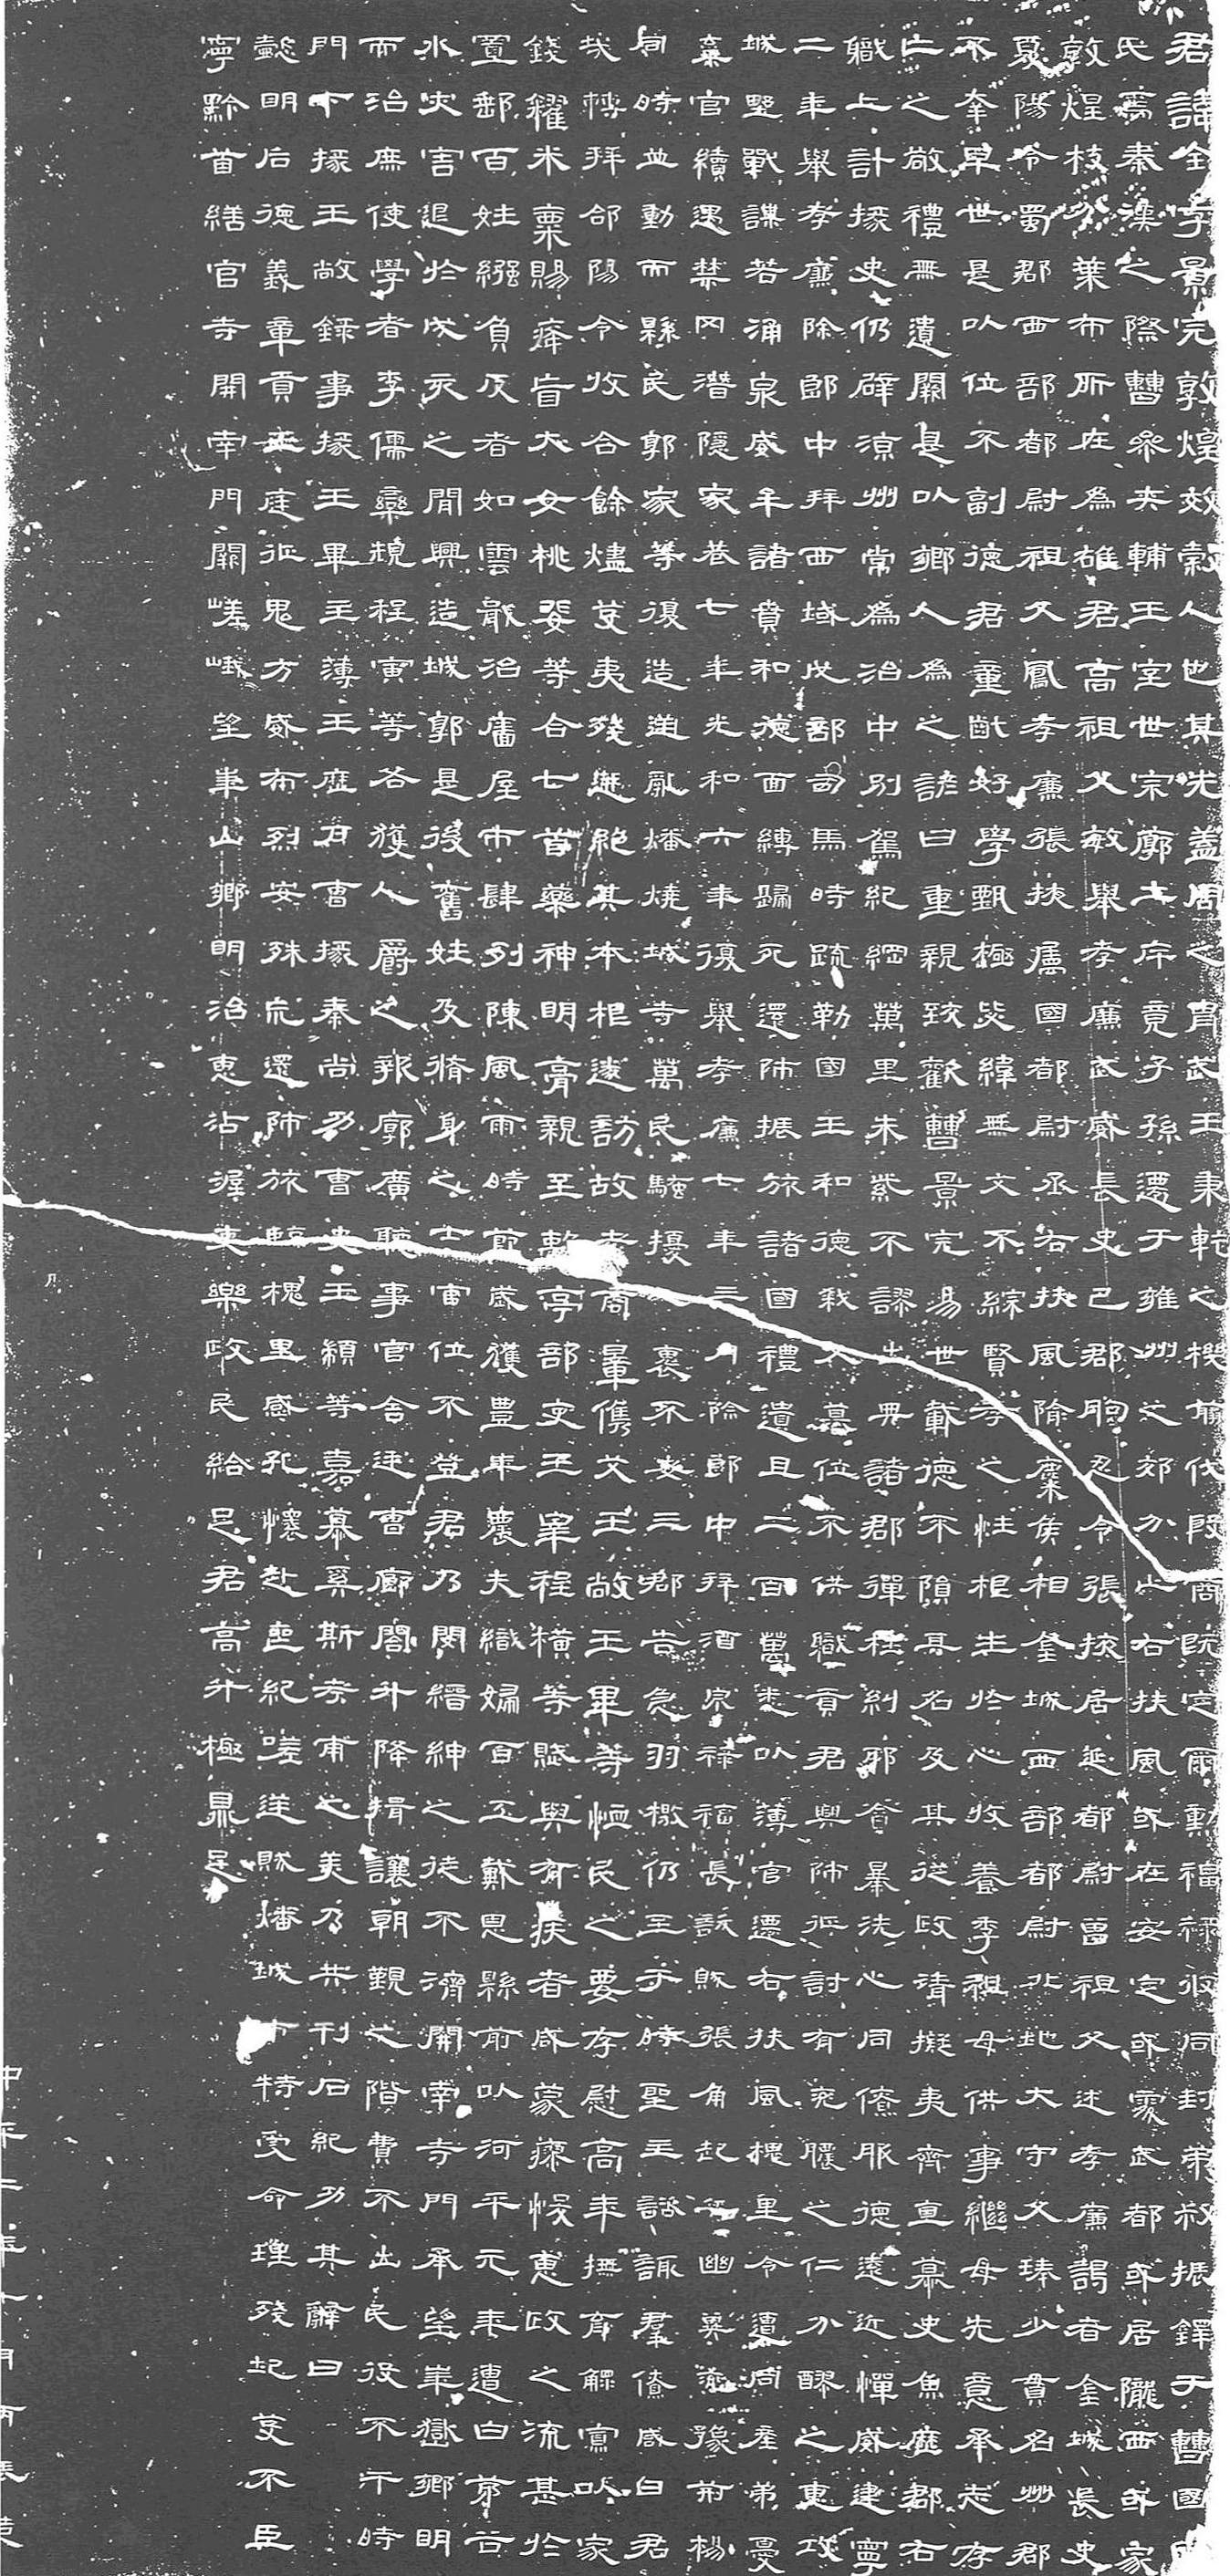
\includegraphics[scale=.32,trim={930pt 1950pt 10pt 25pt},clip]{曹全碑.jpg}
	\tcblower
		\color{white}\hspace{-6.45mm}\vspace{-1.2mm}
		\begin{NiceTabular}[cell-space-limits=4.1pt]{*{7}{W{c}{.1cm}}}
			職 & 亡 & 不 & 夏 & 敦 & 氏 & 君 \\
			上 & 之 & 幸 & 陽 & 煌 & 焉 & 諱 \\
			計 & 敬 & 早 & 令 & 枝 & 秦 & 全 \\
			掾 & 禮 & 世 & 蜀 & 分 & 漢 & 字 \\
			史 & 無 & 是 & 郡 & 葉 & 之 & 景 \\
			仍 & 遺 & 以 & 西 & 布 & 際 & 完 \\
			辟 & 闕 & 位 & 部 & 所 & 曹 & 敦 \\
			涼 & 是 & 不 & 都 & 在 & 參 & 煌 \\
			州 & 以 & 副 & 尉 & 爲 & 夾 & 效 \\
			常 & 鄉 & 德 & 祖 & 雄 & 輔 & 穀 \\
			爲 & 人 & 君 & 父 & 君 & 王 & 人 \\
			治 & 爲 & 童 & 鳳 & 高 & 室 & 也 \\
			中 & 之 & 齔 & 孝 & 祖 & 世 & 其 \\
			別 & 諺 & 好 & 廉 & 父 & 宗 & 先 \\
		\end{NiceTabular}
	\end{boxhorizontalcompare}
	\caption{\content{《曹全碑》片段}{《曹全碑》片段}}
	\footnotesize{\color{darkgray}\content{左為隸書碑文,右為正體字釋文}{左为隶书碑文,右为繁体字释文}}
	\label{figure:《曹全碑》片段}
\end{wrapfigure}
\content{今天人們所用的大部分正體字,其實早在秦漢之時就已基本定型了。以東漢《曹全碑》為例,它是用隸書寫成的。現代人不必專門研習古文字,就可以看懂其中的絕大部分字(\cref*{figure:《曹全碑》片段})。}{今天人们所用的大部分繁体字,其实早在秦汉之时就已基本定型了。以东汉《曹全碑》为例,它是用隶书写成的。现代人不必专门研习古文字,只要能看懂繁体字,就能看懂碑上的绝大部分字(\cref*{figure:《曹全碑》片段})。}\par
\content{但是再往前,面對先秦時期的金文、石鼓文及各種篆文,現代人就看不懂了——別說現代人了,漢朝人也看不懂。那麼,漢人為了釋讀先秦時期殘存的書卷,就不得不專門研究當時的文字。「古文之學」便是這樣興盛起來的。}{但是再往前,面对先秦时期的金文、石鼓文及各种篆文,现代人就看不懂了——别说现代人了,汉朝人也看不懂。那么,汉人为了释读先秦时期殘存的书卷,就不得不专门研究当时的文字。“古文之学”便是这样兴盛起来的。}\par
\content{「古文」是漢朝時出現的概念,一般指\textbf{六國文字}。戰國時期的各國文字本來同源於西周金文,但由於地理隔閡、政治割據等原因,同樣的文字在不同地區可能演變出不同的形態\footnote{一般可以將戰國文字分為五系文字:秦文字、楚文字、三晉文字、齊文字、燕文字。三晉文字並不見得完全統一,但差異較小。}。等到秦滅六國,李斯編定的小篆\footnote{古人通常認為小篆是由李斯創造的,此說未必準確。更有可能的情況是,小篆(以及隸書)的原型在戰國末年就已經出現了,李斯只是完成了整理、𢑥編小篆的工作。}成為全國統一的文字,原來的六國文字便不復使用。漢朝時,同樣源於秦系文字的隸書成為了正體字,於是隨著時間推移,戰國時期的六國文字不再能為一般人所讀解。}{“古文”是汉朝时出现的概念,一般指\textbf{六国文字}。战国时期的各国文字本来同源于西周金文,但由于地理隔阂,政治割据等原因,同样的文字在不同地区可能演变出不同的形态\footnote{一般可以将战国文字分为五系文字:秦文字、楚文字、三晋文字、齐文字、燕文字。三晋文字并不见得完全统一,但差异较小。}。等到秦灭六国,李斯编定的小篆\footnote{古人通常认为小篆是由李斯创造的,此说未必准确。更有可能的情况是,小篆(以及隶书)的原型在战国末年就已经出现了,李斯只是完成了整理、汇编小篆的工作。}成为全国统一的文字,原来的六国文字便不复使用。汉朝时,同样源于秦系文字的隶书成为了正体字,于是随着时间推移,战国时期的六国文字不再能为一般人所读解。}\par
\content{隸書以後,文字形態漸漸穩定下來,後人皆可讀解\footnote{至於草書乃至狂草,那是另一回事了。},所以很少成為人們研究的重點;而古人又不知甲骨文的存在,無從研究更早期的文字。這樣一來,介於金文和小篆之間,而又缺少統一標準,各行其是的六國文字,自然而然地成為古人的研究重點。}{隶书以后,文字形态渐渐稳定下来,后人皆可读解\footnote{至于草书乃至狂草,那是另一回事了。},所以很少成为人们研究的重点;而古人又不知甲骨文的存在,无从研究更早期的文字。这样一来,介于金文和小篆之间,而又缺少统一标准,各行其是的六国文字,自然而然地成为古人的研究重点。}\par
\subsubsection{\content{並行的正體與俗體}{并行的正体与俗体}}
\content{在分裂割據時期,像戰國這樣不同字體並行的情況不足為奇;而在統一王朝時期,不同字體並行的情況也並不鮮見。商代後期有甲骨文和金文並行,秦朝有小篆和隸書並行,西漢則有隸書和章草\footnote{章草,草書的一種,是由隸書演變而來的。我們一般所說的「草書」是指今草,它是由楷書演變而來的。章草與今草有不少差異。}並行,諸如此類。}{在分裂割据时期,像战国这样不同字体并行的情况不足为奇;而在统一王朝时期,不同字体并行的情况也并不鲜见。商代后期有甲骨文和金文并行,秦朝有小篆和隶书并行,西汉则有隶书和章草\footnote{章草,草书的一种,是由隶书演变而来的。我们一般所说的“草书”是指今草,它是由楷书演变而来的。章草与今草有不少差异。}并行,诸如此类。}\par
\content{統一王朝時期並行的字體通常不會有太大差異,相似之處很多\footnote{原因顯而易見。若是要讓甲骨文和現代楷書並行的話,人們要學習兩套全然不同的書寫形式,這樣的並行就只能成為一種負擔。}。就以甲骨文和商代金文來說,它們的寫法大致相似,見\cref*{table:一些漢字的商金文與甲骨文}。}{统一王朝时期并行的字体通常不会有太大差异,相似之处很多\footnote{原因显而易见。若是要让甲骨文和现代楷书并行的话,人们要学习两套全然不同的书写形式,这样的并行就只能成为一种负担。}。就以甲骨文和商代金文来说,它们的写法大致相似,见\cref*{table:一些漢字的商金文與甲骨文}。}\par
\begin{table}[H]
	\centering
	\caption{\content{一些漢字的商金文與甲骨文}{一些汉字的商金文与甲骨文}}
	\label{table:一些漢字的商金文與甲骨文}
	\begin{NiceTabular}{>{\columncolor{gray!50}}c*{6}{c}}[hlines]
		\toprule
		\rowcolor{gray!50}
		\content{現代漢字}{现代汉字} & 天 & 鳥\content{}{(鸟)} & 兒\content{}{(儿)} & 女 & 止 & 韋\content{}{(韦)}\\\midrule[.6pt]
		\Block[m]{}{商金文} & 
\includegraphics[width=3.5em]{金文/天} & 
\includegraphics[width=3.5em]{金文/鳥} & 
\includegraphics[width=3.5em]{金文/兒} & 
\includegraphics[width=3.5em]{金文/女} & 
\includegraphics[width=3.5em]{金文/止} & 
\includegraphics[width=3.5em]{金文/韋}\\
		\Block[m]{}{甲骨文} & 
\includegraphics[width=3.5em]{甲骨文/天} & 
\includegraphics[width=3.5em]{甲骨文/鳥} & 
\includegraphics[width=3.5em]{甲骨文/兒} & 
\includegraphics[width=3.5em]{甲骨文/女} & 
\includegraphics[width=3.5em]{甲骨文/止} & 
\includegraphics[width=3.5em]{甲骨文/韋}\\\bottomrule
	\end{NiceTabular}
\end{table}
\content{比較一下便很容易看出來,金文筆畫流暢,細節豐富,字跡端莊,似是毛筆筆法\footnote{實際上金文不是直接由毛筆寫在青銅器上的,因為青銅器上的銘文都是凹入器皿中的,顯然需要在製造模具時便用某種方式把文字附在模具之上。至於銘文究竟是以何種方式「寫」在青銅器上,這中間又是否有毛筆的參與,今人已不得而知。};甲骨文則是典型的刀筆字,直筆較多,曲筆較少,筆畫轉折處時常拆作兩筆來寫,且每個字的筆畫粗細很一致。}{比较一下便很容易看出来,金文笔画流畅,细节丰富,字迹端庄,似是毛笔笔法\footnote{实际上金文不是直接由毛笔写在青铜器上的,因为青铜器上的铭文者是凹入器皿中的,显然需要在制造模具时便用某种方式把文字附在模具之上。至于铭文究竟是以何种方式“写”在青铜器上,这中间又是否有毛笔的参与,今人已不得而知。};甲骨文则是典型的刀笔字,直笔较多,曲笔较少,笔画转折处时常拆作两笔来写,且每个字的笔画粗细很一致。}\par
\content{書寫工具的差異確實可以解釋一些現象,比如「止」字的甲骨文要比金文簡陋一些。但是它解釋不了,為什麼「韋」的金文是四個「止」,而甲骨文卻只有兩個「止」\footnote{很多甲骨文的寫法不固定。就以「韋」字為例,除了上表所列之字外,筆者還查到有三個「止」的\includecharacter{甲骨文/韋1}和兩個「止」分列左右的\ \includecharacter{甲骨文/韋2}。另外,從西周金文開始,「韋」字便用兩「止」了,寫成\ \includecharacter{金文/韋1},顯然是正體字吸收了俗體字的寫法。}。這種甲骨文比同時期金文簡省部件的現象比比皆是,我們很難牽強附會地把原因歸結為書寫工具的差異。}{书写工具的差异确实可以解释一些现象,比如“止”字的甲骨文要比金文简陋一些。但是它解释不了,为什么“韦”的金文是四个“止”,而甲骨文却只有两个“止”\footnote{很多甲骨文的写法不固定。就以“韦”字为例,笔者还查到有三个“止”的\includecharacter{甲骨文/韋1}和两个“止”分列左右的\ \includecharacter{甲骨文/韋2}。另外,从西周金文开始,“韦”字便用两“止”了,写成\ \includecharacter{金文/韋1},显然是正体字吸收了俗体字的写法。}。这种甲骨文比同时期金文简省部件的现象比比皆是,我们很难牵强附会地把原因归结为书写工具的差异。}\par
\content{真正的原因在於使用埸合。商代青銅器貴重,且生產流程複雜,只能用在比較鄭重的場合下,所以人們「寫」金文時不敢怠慢,要寫得非常標準,更不會為了嫌麻煩而簡省部件。但在日常生活中,人們要使用甲骨及竹簡書寫大量內容,自然會對筆畫繁複的字感到厭煩,於是有意或無意地簡省部件,只要保證還能看懂即可。用於正式場合的\textbf{正體}和用於非正式場合的\textbf{俗體}便是這樣分道揚鑣的。}{真正的原因在于使用场合。商代青铜器贵重,且生产流程复杂,只能用在比较郑重的场合下,所以人们“写”金文时不敢怠慢,要写得非常标准,更不会为了嫌麻烦而简省部件。但在日常生活中,人们要使用甲骨及竹简书写大量内容,自然会对笔画繁复的字感到厌烦,于是有意或无意地简省部件,只要保证还能看懂即可。用于正式场合的\textbf{正体}和用于非正式场合的\textbf{俗体}便是这样分道扬镳的。}\par
\content{秦朝以小篆為正體,官方文件皆使用小篆。隸書的書寫效率高於小篆,所以底層公務員們當然願意使用隸書,隸書便是秦朝的俗體。到了西漢,隸書逐漸取代小篆,成為正體;而由隸書發展而來的、書寫效率更高的章草則作為俗體存在。唐朝及以後的正體一般都是楷書,而俗體主要是行書。}{秦朝以小篆为正体,官方文件皆使用小篆。隶书的书写效率高于小篆,所以底层公务员们当然愿意使用隶书,隶书便是秦朝的俗体。到了西汉,隶书逐渐取代小篆,成为正体;而由隶书发展而来的、书写效率更高的章草则作为俗体存在。唐朝及以后的正体一般都是楷书,而俗体主要是行书。}\par
\content{\cref{appendix:evolution of chinese characters}是筆者根據各種資料整理而成的漢字演變圖譜,可供讀者參考。}{\cref{appendix:evolution of chinese characters}是笔者根据各种资料整理而成的汉字演变图谱,可供读者参考。}\par
% \subsection{\content{二簡字}{二简字}}
% \begin{boxquote}{\content{裘錫圭《文字學概要》}{裘锡圭《文字学概要》}}
% 	\content{為了把象形的古文字改造成隶、楷而破壞一部分字的結構,是迫不得已的,也是值得的。在楷書早已成熟的情況下,仅仅為了減少筆畫而去破壞某些字的結構,把它們變成記號字,這樣做究竟是不是必要,是不是值得,就大可懷疑了。}{为了把象形的古文字改造成隶、楷而破坏一部分字的结构,是迫不得已的,也是值得的。在楷书早已成熟的情况下,仅仅为了减少笔画而去破坏某些字的结构,把它们变成记号字,这样做究竟是不是必要,是不是值得,就大可怀疑了。}
% \end{boxquote}
